\documentclass[a4paper,twoside,10pt]{article}
% Richard Klein (2020,2021)

% Include Packages
%\usepackage[a4paper,inner=3.5cm,outer=2.5cm,top=2.5cm,bottom=2.5cm]{geometry}  % Set page margins
\usepackage{fullpage}
\usepackage{float}                  % Allows 'Here and Only Here' [H] for Floats
\usepackage{url}                    % \url{} command
\usepackage{charter}                  % Set font to Times
\usepackage{graphicx}               % \includegraphics
\usepackage{subfigure}              % Allow subfigures
\usepackage{wrapfig}
\usepackage{amsmath}
\usepackage{amssymb}
\usepackage{multicol}
\usepackage{amsthm}
\usepackage{booktabs}
\usepackage{parskip}
\usepackage{setspace}
\usepackage[all]{nowidow}
\setnoclub[2]
\setnowidow[2]
\graphicspath{ {./images/} }
% Referencing
% Provides \Vref and \vref to indicate where a reference is.
\usepackage{varioref} 
% Hyperlinks references
\usepackage[bookmarks=true,bookmarksopen=true]{hyperref} 
% Provides \Cref, \cref, \Vref, \vref to include the type of reference: fig/eqn/tbl
\usepackage{cleveref} 
% Setup Hyperref
\hypersetup{
  colorlinks   = true,              %Colours links instead of ugly boxes
  urlcolor     = blue,              %Colour for external hyperlinks
  linkcolor    = blue,              %Colour of internal links
  citecolor    = blue                %Colour of citations
}
% Names for Clever Ref
\crefname{table}{table}{tables}
\Crefname{table}{Table}{Tables}
\crefname{figure}{figure}{figures}
\Crefname{figure}{Figure}{Figures}
\crefname{equation}{equation}{equations}
\Crefname{equation}{Equation}{Equations}

% Wits Citation Style
\usepackage{natbib} % Force natbib.sty to put citation labels in the reference list
\makeatletter
\renewcommand\NAT@biblabel[1]{\def\citeauthoryear##1##2{##1 ##2}[#1]\hfill}
\renewcommand\NAT@bibsetup[1]{%
  \setlength{\itemsep}{\bibsep}\setlength{\parsep}{\z@}}
\def\@lbibitem[#1]#2{%
  \if\relax\@extra@b@citeb\relax\else
    \@ifundefined{br@#2\@extra@b@citeb}{}{%
     \@namedef{br@#2}{\@nameuse{br@#2\@extra@b@citeb}}}\fi
   \@ifundefined{b@#2\@extra@b@citeb}{\def\NAT@num{}}{\NAT@parse{#2}}%
   \item[\hfil\hyper@natanchorstart{#2\@extra@b@citeb}\@biblabel{#1}%
    \hyper@natanchorend]%
    \NAT@ifcmd#1(@)(@)\@nil{#2}}
\makeatother


\bibliographystyle{named-wits}
\bibpunct{[}{]}{;}{a}{}{}  % to get correct punctuation for bibliography
\setlength{\skip\footins}{1.5cm}
\newcommand{\citets}[1]{\citeauthor{#1}'s \citeyearpar{#1}}
\renewcommand\bibname{References}  

\pagestyle{plain}
\pagenumbering{roman}

\begin{document}
\onecolumn
\singlespacing
\thispagestyle{empty}
\setcounter{page}{-1}
\addcontentsline{toc}{chapter}{Preface}
\
\begin{center}
  \vfill
  {
  \huge \textsc{Computer Science Honours}\\
  \huge \textsc{ACML Assignment Report}\\
  \vspace{20mm}
  \huge \bf \textsc{Machine Learning in Identifying Handwritten Digits}\\
  \vspace{5mm}
  \large School of Computer Science \& Applied Mathematics\\
  \large University of the Witwatersrand\\[20pt]
  \today \\
  \vspace{5mm}
  \normalsize
  Aaqib Khan - 2359325\\[10pt]
  Katlego Kungoane - 2320690\\[10pt]
  Musawenkosi Gumpu - 2326254\\[10pt]
  Verushan Naidoo - 2374896
  }

  \vfill
  
\includegraphics[width=1.5cm]{wits}
  \vspace{10pt}\\
  \small{A report submitted to the Faculty of Science, University of the Witwatersrand, Johannesburg,
in partial fulfilment of the requirements for the degree of Bachelor of Science with Honours}\\
\end{center}
\vfill
\newpage

\pagestyle{plain}
\setcounter{page}{-1}
\newpage
\pagenumbering{arabic}

\section{Introduction}
Handwritten digit classification plays a pivotal role in various fields, ranging from optical character recognition to digitized archival systems. With the ever-increasing digitization of information, accurate and efficient techniques for automated digit recognition are essential. In recent years, machine learning algorithms have emerged as powerful tools for tackling this challenging task, exhibiting remarkable capabilities in recognizing and classifying handwritten digits.

This report presents a comprehensive comparison of Neural Networks and Convolutional Neural Networks (CNNs) in the context of handwritten digit classification. Each of these algorithms has their unique characteristics, advantages, and limitations, making them suitable candidates for exploring the intricate patterns and features of handwritten digits.

In this comparative analysis, we aim to evaluate the performance of these three approaches in terms of accuracy, computational efficiency, and generalization capabilities. We will employ a well-known handwritten digit dataset called MNIST (Modified National Institute of Standards and Technology) dataset, which consists of a large collection of labeled handwritten digit images, serving as our benchmark for evaluating the classification models.

The report is structured as follows: In Section \ref{sec:model_choice}, the model choices are discussed and motivated as well as providing reasons as to why other common models were not explored. Section \ref{sec:experimental_setup} details the experimental setup, including the pre-processing steps, model architectures, and evaluation metrics used. Furthermore, in Section \ref{sec:experimental_setup} we present the results obtained from the experiments and analyzes the performance of each algorithm as well as variants of the same algorithm.

By conducting this comparative analysis, we aim to shed light on the strengths and weaknesses of Neural Networks and Convolutional Neural Networks in the context of handwritten digit classification. This study will contribute to the existing body of research, providing valuable insights for researchers, practitioners, and enthusiasts interested in exploring the performance and trade-offs of different machine learning algorithms for this specific task.

\section{Model Choices}
\label{sec:model_choice}
Convolutional neural networks (CNNs) and neural networks (NNs) were chosen as better candidates for identifying handwritten digits over Naive Bayes and decision forest models due to their unique capabilities. CNNs excel in image processing tasks by leveraging their convolutional layers, which extract features hierarchically, allowing them to capture local patterns and spatial relationships in the data. This is crucial for recognizing intricate details in handwritten digits. Moreover, CNNs employ parameter sharing, reducing the number of parameters and making them more efficient for image classification tasks. On the other hand, NNs offer a broader range of expressiveness and flexibility compared to Naive Bayes models and decision forests. They can learn complex nonlinear relationships between input features and output labels. Handwritten digits exhibit various characteristics and nuances that can be better captured by the nonlinear transformations and hidden layers of NNs, enhancing their ability to accurately classify and distinguish different digits. Even though neural networks are dependant on consistent patterns and may incorrectly identify numbers if the digits are slightly angled for example. Even with this weakness, neural networks should still be able to learn a pattern for handwritten digits that are more or less similar in size and orientation.

Naive Bayes and Decision Forests are both popular machine learning algorithms used for classification tasks, including recognizing handwritten digits. However, they may face challenges when it comes to identifying handwritten digits due to certain limitations.

\subsection{Naive Bayes}
Naive Bayes is a probabilistic algorithm that makes an assumption of independence among the features. When applied to handwritten digit recognition, it treats each pixel of the image as a separate feature. This assumption can be problematic because neighboring pixels in a digit image are often highly correlated and carry important spatial information. Ignoring this correlation can result in a loss of accuracy when distinguishing between different digits that have similar shapes but differ in pixel arrangements.

Additionally, Naive Bayes assumes that all features are equally informative and independent of each other given the class label. In the case of handwritten digit recognition, this assumption may not hold true. Certain features or combinations of features may be more relevant for distinguishing between certain digits, and Naive Bayes may struggle to capture such complex dependencies.

\subsection{Decision Forests}
Decision Forests, also known as Random Forests, are ensemble learning methods that combine multiple decision trees to make predictions. Each decision tree is trained on a random subset of the data and features. While Decision Forests are generally effective for classification tasks, they can encounter difficulties with handwritten digit recognition due to the following reasons:
\begin{enumerate}
    \item Variability in writing styles: Handwriting can vary significantly among individuals, and even a single person's writing can differ slightly between instances. This variability poses a challenge because Decision Forests rely on learning distinct decision boundaries between classes. If the writing styles exhibit substantial variations within the same digit class, the decision boundaries may become less accurate, leading to mis-classifications.
    \item Over-fitting or under-fitting: Decision Forests can be prone to over-fitting or under-fitting the data. Over-fitting occurs when the model captures noise or irrelevant details in the training data, leading to poor generalization. Under-fitting, on the other hand, happens when the model is too simplistic and fails to capture the underlying patterns in the data. Handwritten digit recognition requires a balance between capturing the complexity of different digit shapes and avoiding over-fitting or under-fitting, which can be challenging to achieve with Decision Forests.
\end{enumerate}

While Naive Bayes and Decision Forests are versatile algorithms, they may struggle with identifying handwritten digits due to the limitations of Naive Bayes assumptions regarding feature independence and the challenges posed by the variability and complexity of handwritten digit data for Decision Forests. These are the main reasons as to why CNNs and NNs have been chosen for the models that are to be explored.

\section{Experimental Setup}
\label{sec:experimental_setup}

\subsection{Dataset}
There are a total of $284642$ data points that are going to be used. This large data-set will provide many benefits in terms of learning. Some of these benefits include:
\begin{itemize}
    \item \textbf{Improved Model Generalization:} The ability to generalize can be enhanced with larger data sets. The model can learn to capture a wider range of patterns with more varied and diversified samples, lowering the likelihood of over-fitting. This makes the model more dependable and robust by allowing it to perform better on unobserved data.

    \item \textbf{Increased Model Accuracy:} More data implies the model has more information to learn from. The model may better comprehend the underlying patterns and relationships in the data by training on a larger data-set, which improves prediction accuracy and overall performance.

    \item \textbf{Better Representation of the Underlying Population:} A larger data-set might offer a sample that is more representative of the population or distribution on which the data are based. This can lessen bias and increase the model's capacity to predict the target population correctly.
\end{itemize}

\subsection{Pre-processing}
Since our data is simply a collection of images, there is not much insight to gain from using exploration strategies like a distribution plot, or a covariance matrix. What we can show you is a graphic of some of the images that we are using.

The following pre-processing steps were applied:
\begin{itemize}
    \item \textbf{Image Acquisition:} The dataset used for handwritten digit recognition is a compilation sourced from various datasets. The primary dataset utilized is the well-known MNIST dataset \cite{deng2012mnist,Colianni2017}. Additionally, supplementary datasets obtained from Kaggle have been incorporated, featuring diverse handwritten digit samples. These include Japanese handwritten digits provided by Keio University \cite{Zalek2019}, self-generated numbers with varying backgrounds and positions \cite{V2022}, and Swiss handwritten digits \cite{Meier2023}. Furthermore, a dataset by \citet{Heusser2020} is utilized, which includes digits and simple mathematical operators. It is important to note that the focus of the project remains primarily on the recognition of handwritten digits and not the included mathematical operators. 
    \item \textbf{Image Re-scaling:} The images are resized to a consistent size. In our case, the images are resized to $28 \times 28$.
    
    \item \textbf{Gray-scale Conversion:} Convert the images to gray-scale if they are not already in gray-scale format. This reduces the dimensionality and simplifies subsequent analysis.
    
    \item \textbf{Thresholding:} In the case of handwritten digits, there are only two properties of an image that we really care about. These are the foreground and background pixels. Therefore, we only require pixels to either be classified as a foreground or a background pixel. Therefore we apply a thresholding operation to convert the gray-scale images into binary images. The thresholding levels are chosen to also eliminate low and high noise levels that may be present in the image.

    \item \textbf{Label Encoding:} A numerical label is assigned to each handwritten digit. For example, map the digit "$0$" to label $0$, "$1$" to label $1$, and so on. This step is crucial for supervised learning tasks, as it converts the output into a format that can be used to train our models.
    
    \item \textbf{Data splitting:} Split the pre-processed data-set into training and testing subsets. The training set is used to train the machine learning model, while the testing set is used to evaluate its performance. We have used a $60, 20, 20$ split amongst training, validation and testing data respectively. 
\end{itemize}

\begin{figure}[H]
    \centering
    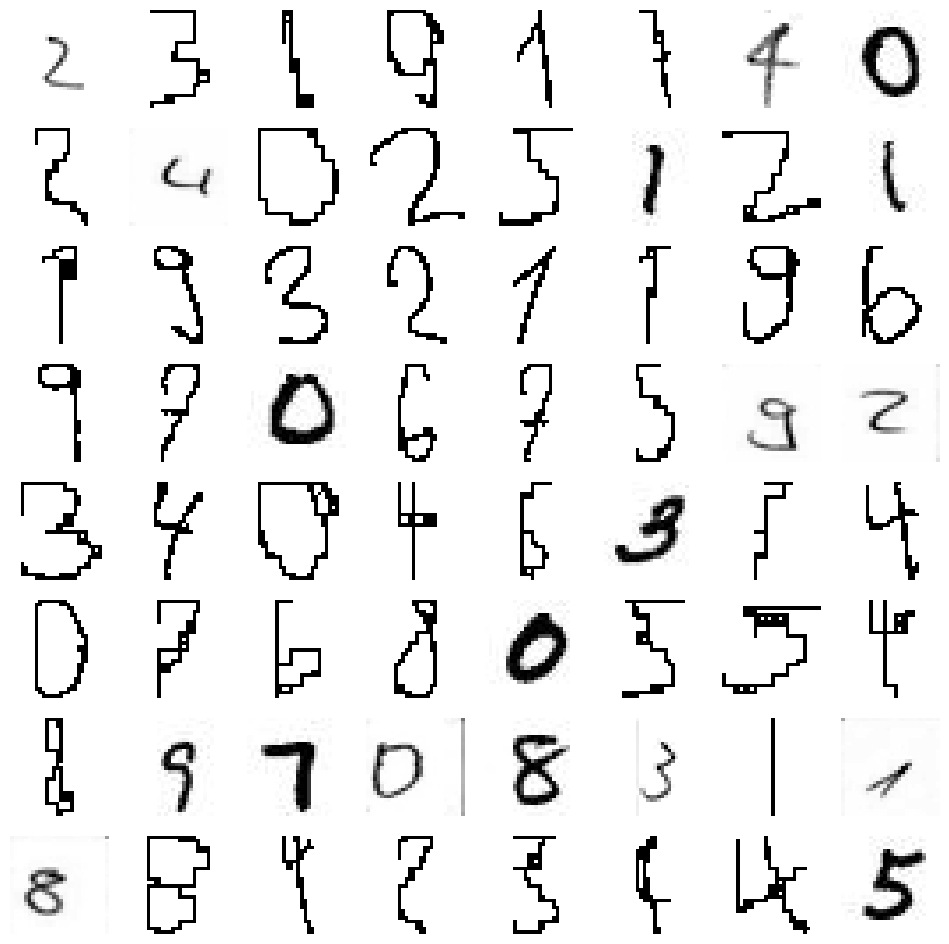
\includegraphics[scale=0.25]{data_visual}
    \caption{Visualisation of handwritten digits}
    \label{fig:data_visual}
\end{figure}

\subsection{Activation Functions}
Activation functions serve as a non-linear function which allows neural networks and convolutional neural networks to learn more sophisticated features. The activation functions used in our model designs are as follows:

\begin{itemize}
    \item \textbf{ReLu:} $f(x) = \max{(0, x)}$
    \item \textbf{Log Softmax:} $g(\overline{o}) = \overline{o} - \log{\sum_{i=1}^{K}{(\overline{o_i})}}$\\
    where:
    \begin{itemize}
        \item $o$ represents the values at the output layer
        \item $o_i$ represents the $i$'th value in $\overline{o}$
        \item $k$ represents number of nodes in the output layer $\overline{o}$
    \end{itemize}
\end{itemize}

\subsection{Loss functions}
Loss functions, also known as cost functions, are critical components of neural networks. Their goal is to quantify the difference between a neural network's anticipated output and the true or desired output. Loss functions provide feedback signals to the learning process and serve as a measure of how effectively the network is working.

The following loss functions will be used, noting that $y_i$ is the predicted class, $t_i$ is the target class corresponding to the evaluated datapoint:
\begin{itemize}
	\item \textbf{Cross-Entropy Loss: } $L_{CE} = -\sum_i (y_i - t_i)$
	\item \textbf{Mean Square Error: } $MSE = \frac{1}{n}\sum_i (y_i - t_i)^2$
	\item \textbf{Negative Log Likelihood: } $NLL = -log(p(y_t))$, where $p(y_t)$ is the likelihood that the predicted class is the target class.
\end{itemize}

\subsection{Convergence}
Convergence refers to the process by which a model gradually improves its performance across training iterations until it achieves a desirable state. More specifically, it means that the loss function of the model is falling and nearing a minimum, indicating that the model is approaching the optimal set of parameters.

The model modifies its parameters during training depending on the gradients of the loss function with respect to those parameters. Typically, optimization procedures such as gradient descent are used to accomplish the changes. Speed of convergence is an important factor when analysing models as it gives insight into the generalization skills of a model.

To ensure convergence during the training process, we monitored the change in accuracy between epochs by evaluating the model's performance on the validation dataset. Based on our analysis, we determined that convergence was achieved when the difference in validation accuracy became smaller than 0.0025\%. This allowed us to establish when the model had reached a stable and satisfactory level of performance.

\subsection{Optimizers}
Optimizers are techniques or approaches used to improve a model's performance by altering its parameters throughout the training process. An optimizer's purpose is to minimize the loss function and discover the best values for the model's parameters to get the best performance on the given task.

An optimizer iteratively modifies the model's parameters during training based on the gradients of the loss function with respect to those parameters. These gradients reflect the amount and direction of the steepest decline towards the loss function's minimum. The optimizer steers the model to the optimal parameter values by altering the parameters in the opposite direction as the gradients.

The following optimizers will be used:
\begin{itemize}
    \item \textbf{SGD:} Stochastic gradient descent is an iterative method for optimizing an objective function with appropriate properties. It is a stochastic approximation of gradient descent optimization because it replaces the actual gradient (derived from the whole data set) with an estimate of the gradient (calculated from a randomly selected portion of the data).

    \item \textbf{RMS:} RMSprop (Root Mean Square Propagation) is an additional adaptive optimization approach. To change the learning rate, it employs an exponentially decaying average of squared gradients. During training, RMSprop prevents the learning rate from getting too slow.

    \item \textbf {Adam:} Adam (Adaptive Moment Estimation) is a hybrid adaptive optimization technique that has the advantages of RMSprop. It adjusts the learning rate for each parameter based on estimates of the gradients' first moment (mean) and second moment (uncentered variance). Adam is well-known for its robustness and speed of convergence.
\end{itemize}

\subsection{Performance Metrics}
A model's metrics indicate that the model has performed very well on training data as well as the testing data. The closeness between the metrics shown in the table above indicate that the model is functioning consistently across all evaluation aspects without any noticeable bias to any specific metric.


The metrics that will be used are:
\begin{itemize}
    \item \textbf{Accuracy } $=\frac{\text{Total Number of Samples}}{\text{Number of Correctly Predicted Samples}}$
    \item \textbf{Precision } $= \frac{\text{True Positives}}{\text{True Positives + False Positives}}$
    \item \textbf{Sensitivity } $= \frac{\text{True Positives}}{\text{True Positives + False Negatives}}$
    \item \textbf{F1 Score } $= 2 \times \frac{\text{Precision} \times \text{Sensitivity}}{\text{Precision} + \text{Sensitivity}}$
\end{itemize}



\subsection{Neural Networks}
\subsubsection{Input and Output format}
Neural networks require an flattened input layer of values. Since the data has been sized to be a $28 \times 28$ grid, we will reshape the data to a $1D$ array of $784$ elements. This flattened data can now be propagated through the network in order for the the network to learn from the input data.

In the case of the output layer, we would like the network to classify a data point as one of 10 possible digits from $0$ till $9$. Therefore we have $10$ output neurons. These output neurons will represent the probability of each digit matching the data point. In order to find the classification suggested by the network, we simply take the index of the maximum output node. 

\subsubsection{Baseline Network}
This baseline neural network is a small network which will be used as a base for bench-marking.

\begin{figure}[H]
	\centering
	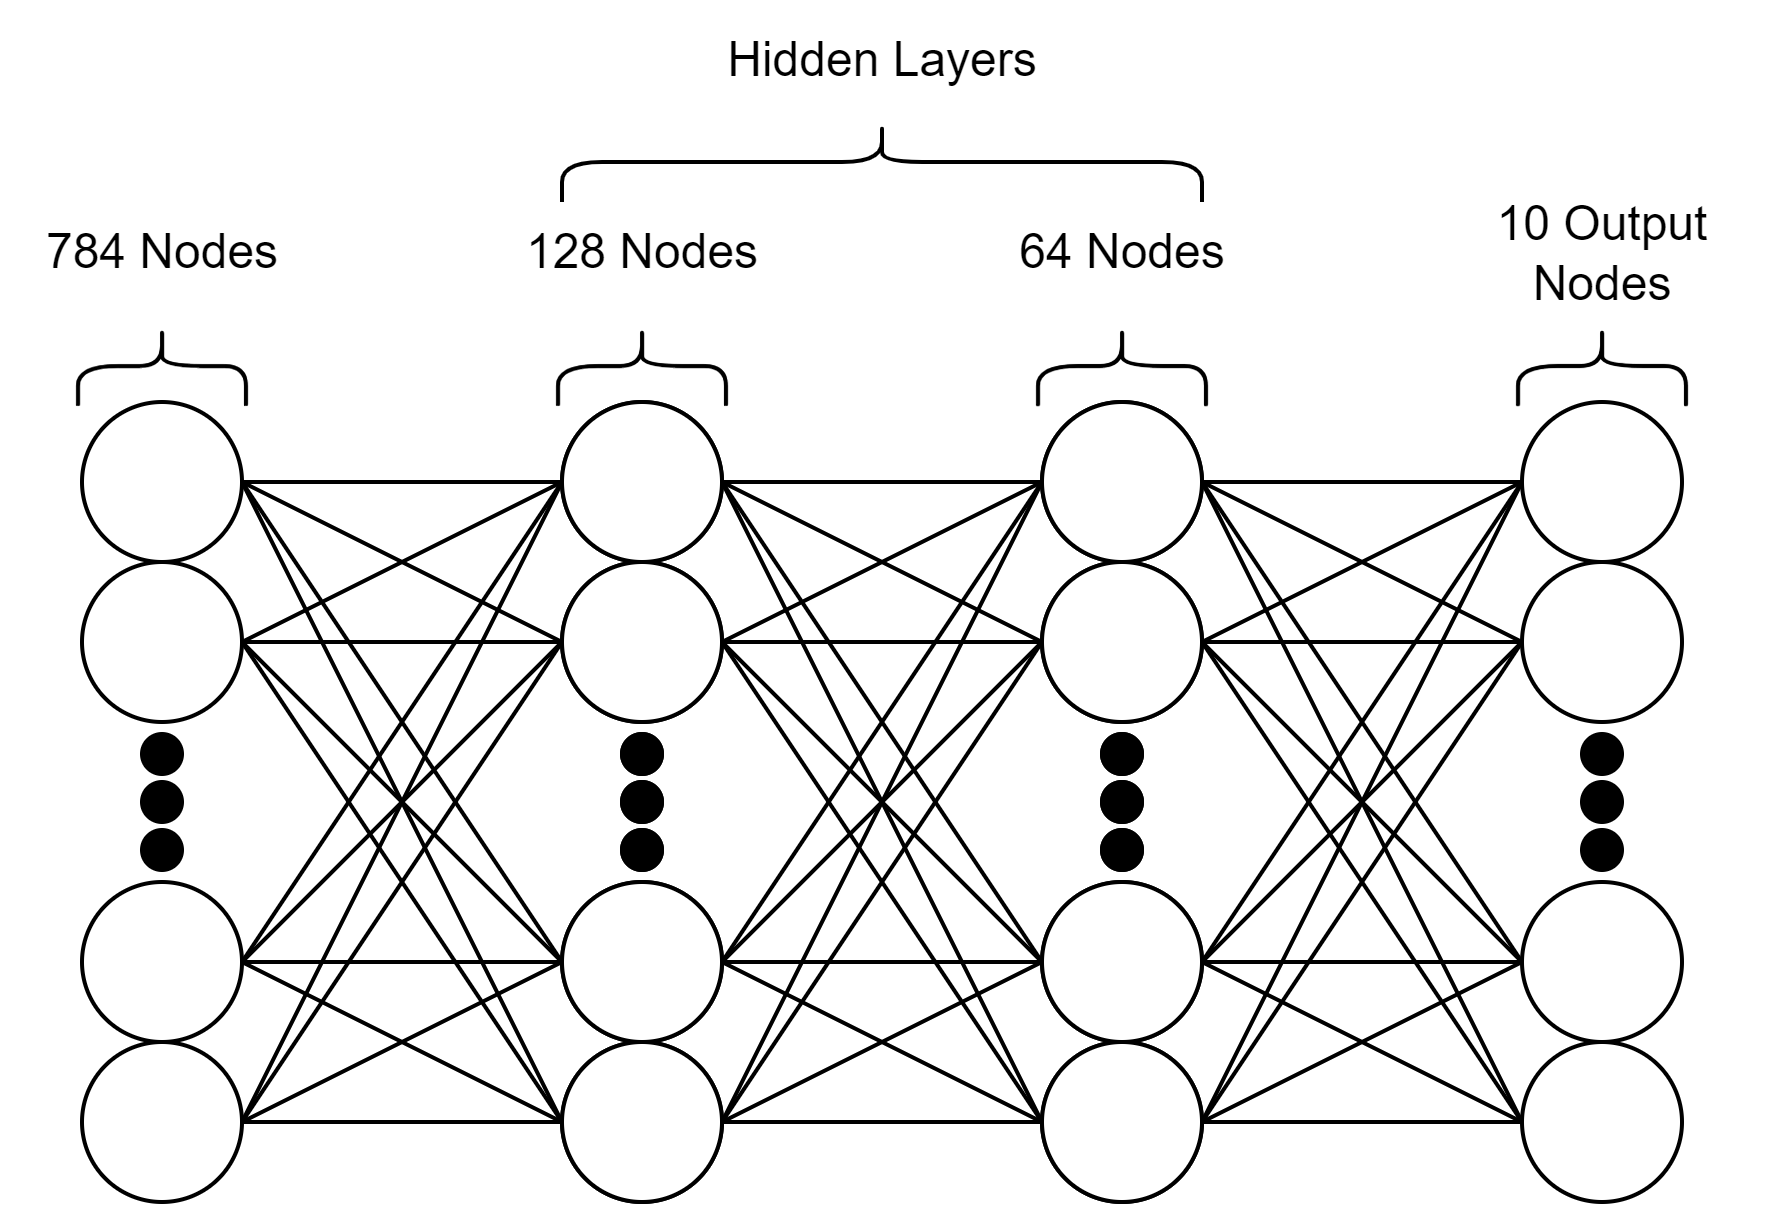
\includegraphics[scale=0.5]{Baseline_NN}
	\caption{Visualisation of the Neural Network}
	\label{fig:baseline_nn}
\end{figure}

Our baseline model contains the following properties:
\begin{itemize}
    \item $2$ hidden layers using Relu and Relu Softmax activation functions in their respective layers.
    \item $128$ and $64$ nodes for the hidden layers respectively.
    \item The loss value is determined by the negative least likelihood loss function.
\end{itemize}

The baseline neural network has performed as follows:

\begin{figure}[H]
    \begin{minipage}{0.5\linewidth}
        \centering
        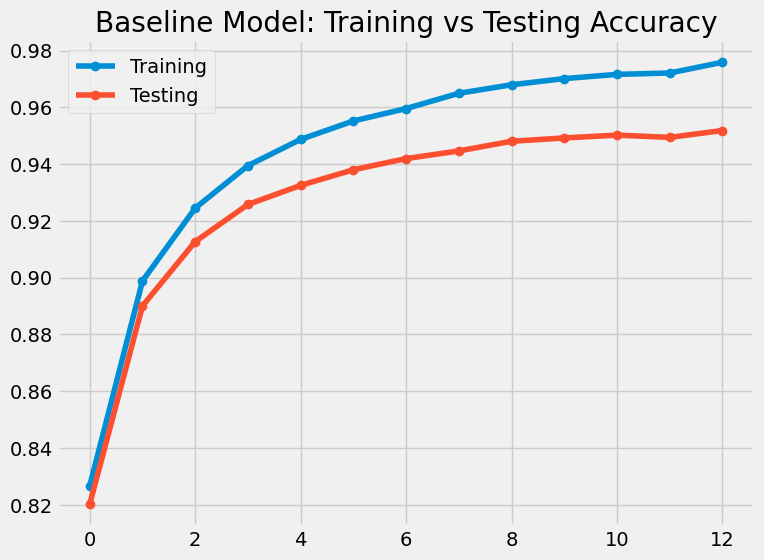
\includegraphics[scale=0.3]{Baseline Acc}
    \end{minipage}\hfill
    \begin{minipage}{0.5\linewidth}
        \centering
        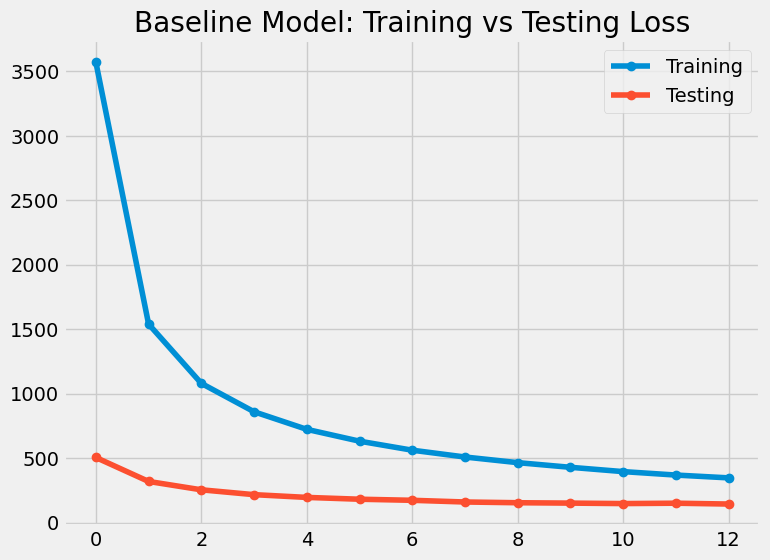
\includegraphics[scale=0.3]{Baseline Loss}
    \end{minipage}\hfill
    \caption{The accuracy and loss improvement respectively over $12$ epochs}
    \label{fig:baseline_graph_perf}
\end{figure}

It should be noted that the macro-precision, macro-sensitivity and macro-F1 scores were evaluated, to ensure uniformity.
The performance metrics of this simple neural network are as follows:
\begin{center}
\begin{tabular}{||c|c||}
    Accuracy & $0.9518$ \\
    Precision & $0.9519$ \\
    Sensitivity & $0.9520$ \\
    F1 Score & $0.9519$ \\
\end{tabular}
\end{center}

The close similarity amongst the evaluation metrics indicate that the model structure is reliable, making accurate predictions without any significant bias towards specific classes.

Here are some mis-classifications from the baseline model:
\begin{figure}[H]
    \centering
    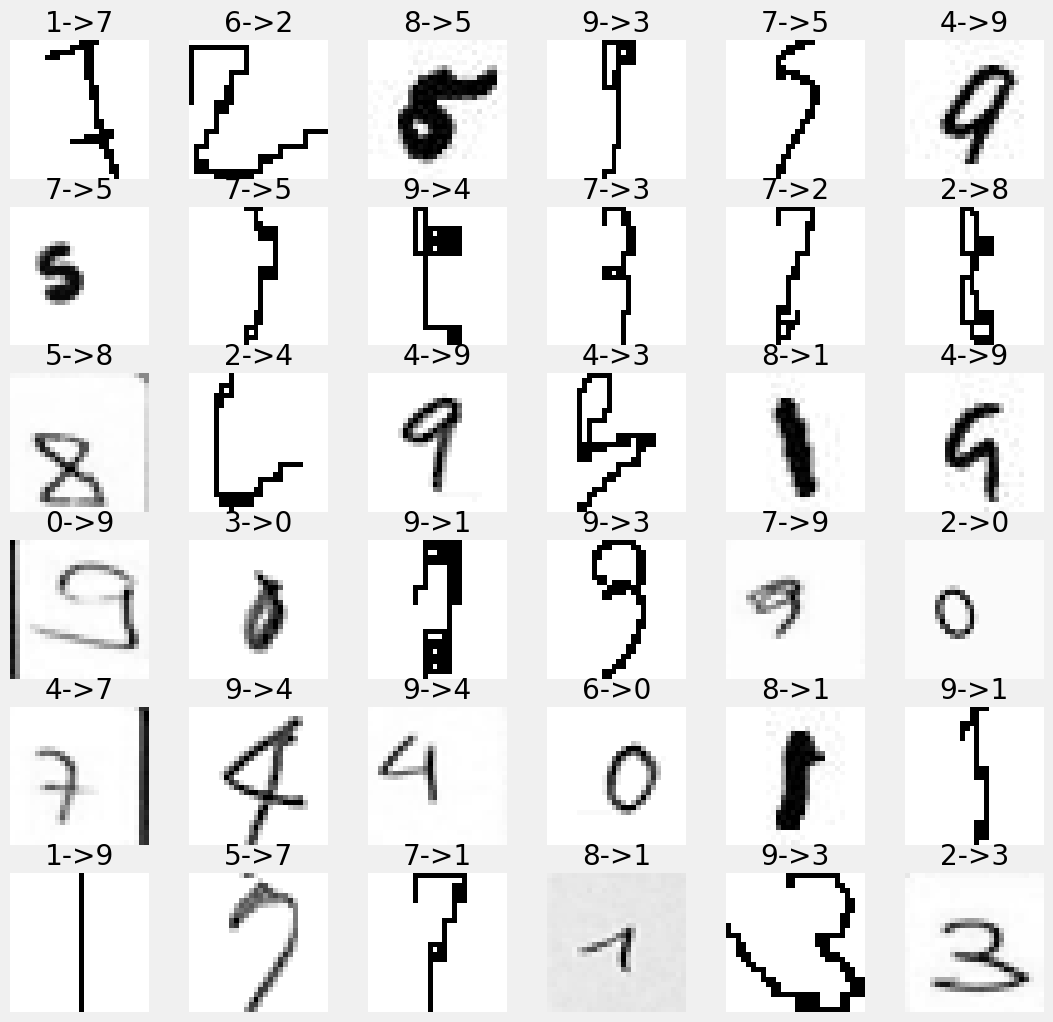
\includegraphics[scale=0.3]{Baseline_incorrect}
    \caption{Incorrect classifications in the format prediction $\rightarrow$ actual}
    \label{fig:baseline_incorrect}
\end{figure}

While our model achieves high overall accuracy, we have observed instances of obvious misclassifications for certain digits that are visually distinct and easily recognizable. For example, we have noticed cases where the digit "0" is misclassified as a "2". To address this issue, we propose two potential improvements to enhance the model's performance:

Dataset refinement: One approach is to reduce the dataset by excluding samples that are deemed illegible. For instance, we can remove instances where the digit "4" is misinterpreted as a "9". By removing such problematic samples, we can mitigate the noise that the model learns from and help improve its ability to correctly predict obvious digits.

Additional legible datasets: Another strategy is to introduce supplementary datasets that contain more legible instances of specific digits, particularly those that tend to be misclassified due to their similarity in stroke patterns. In particular, providing more well-defined examples of digits "0" and "9", as well as "2" and "3", can help the model better differentiate between these pairs, as their strokes share similar characteristics. This additional training data can help the model learn more discriminative features and enhance its ability to correctly classify these challenging digit pairs.

By implementing these improvements, we aim to reduce the occurrence of misclassifications for obvious digits and enhance the overall performance and accuracy of our model.

\subsubsection{Different Network Configurations}
In this performance test, we will use four network configurations. Each of these network configurations have varying hidden layer counts as well as different node counts per hidden layer. These networks will be analysed to identify if there's any benefit to having smaller or larger networks in terms of number of hidden layers or the number of nodes per layer.

These four networks are structured as follows:
\begin{table}[H]
    \centering
    \begin{tabular}{||c|c|c|c|c||}
    \hline
    & Tiny Network & Small Network & Large Network & Massive Network \\
    \hline
    \hline
    Hidden layer count & $1$ & $2$ & $4$ & $4$ \\
    \hline
    Hidden layer node counts & $36$ & $36, 6$ & $256, 128, 64, 16$ & $1024, 512, 256, 128$ \\
    \hline
    \end{tabular}
\end{table}

All networks will use a ReLu activation function for all hidden layers except the last hidden layer which will use a Log Softmax activation function.

\begin{figure}[H]
    \centering
    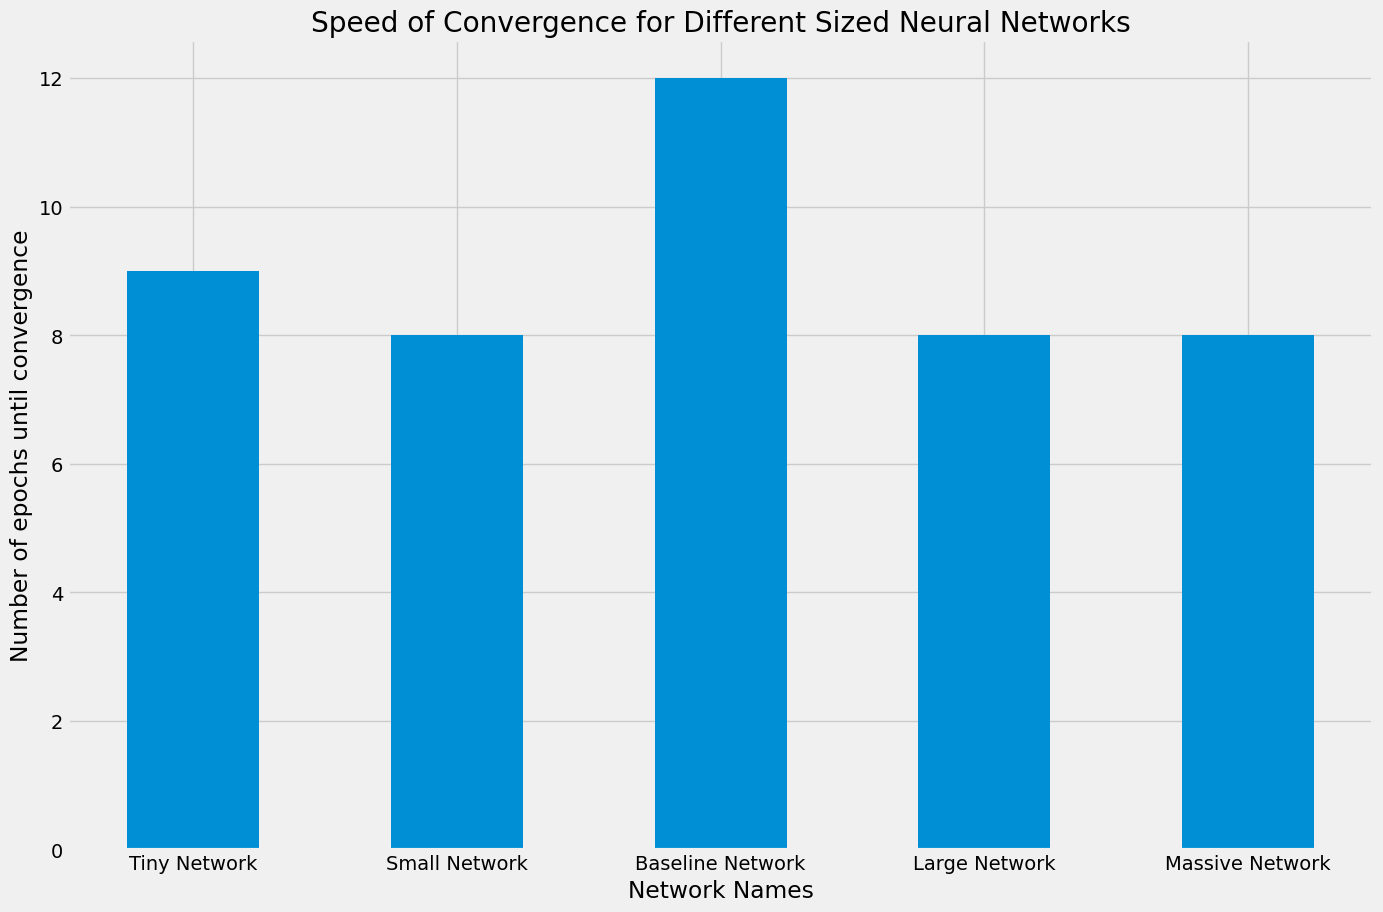
\includegraphics[scale=0.3]{Convergence NN}
    \caption{Epochs required for convergence for each of the different network configurations}
    \label{fig:nn_convergence}
\end{figure}

\begin{figure}[H]
    \centering
    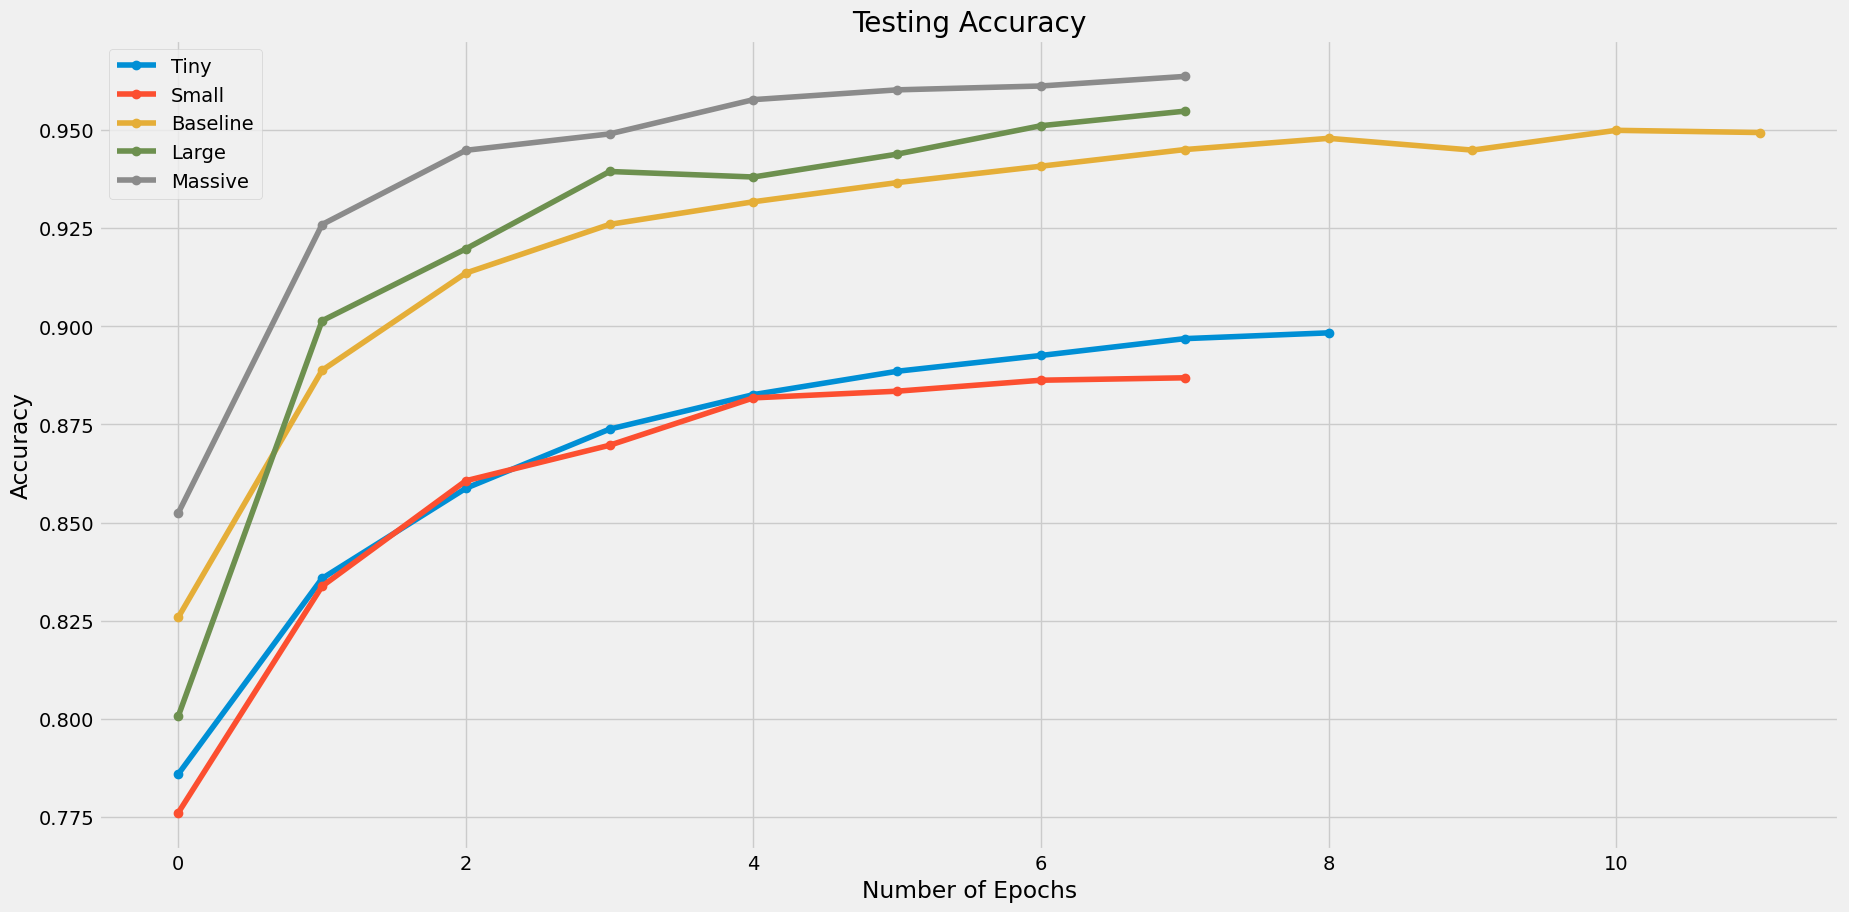
\includegraphics[scale=0.3]{Multiple Model Accuracy}
    \caption{Model accuracy on training data for each network configuration}
    \label{fig:nn_model_accuracy}
\end{figure}

We can see that all of the network configurations do very well on this data-set with all network configurations getting above $85\%$ accuracy once convergence has been reached. We do notice that allowing for less variance in the model does result in a less accurate model. This is mainly due to the model underfitting the data. These models will now be tested against unseen data in order to test their ability to generalize. 

\begin{figure}[H]
    \centering
    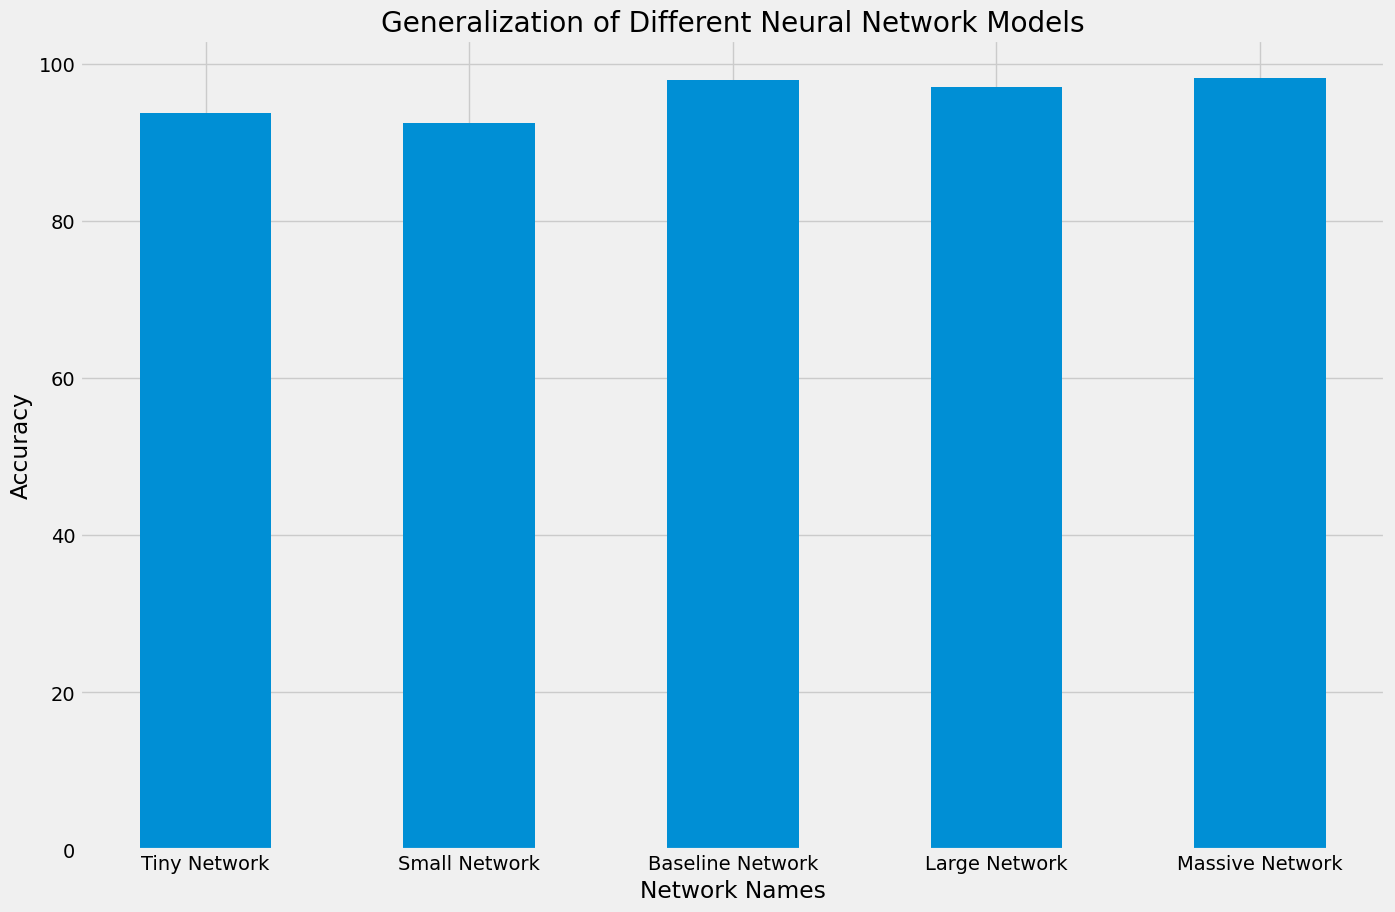
\includegraphics[scale=0.3]{NN_test_Generalization}
    \caption{Model accuracy on test data for each network configuration}
    \label{fig:nn_test_generalization}
\end{figure}

Based on the results shown in Figure \ref{fig:nn_test_generalization}, it can be seen that all of the models perform well on unseen data which also means that there is little to no over-fitting. This is also most likely due to having such a large data-set which ensures that no biases are developed during training.

\subsubsection{Loss Function Optimization}
Loss functions affect the way the network perceives it's error. Therefore, it of great interest to measure how much of a difference various loss functions make to the overall performance of neural networks.

The loss functions that will be evaluated are:
\begin{itemize}
    \item Mean Square Error
    \item Cross Entropy
    \item Negative Log Likelihood
\end{itemize}

\begin{figure}[H]
    \centering
    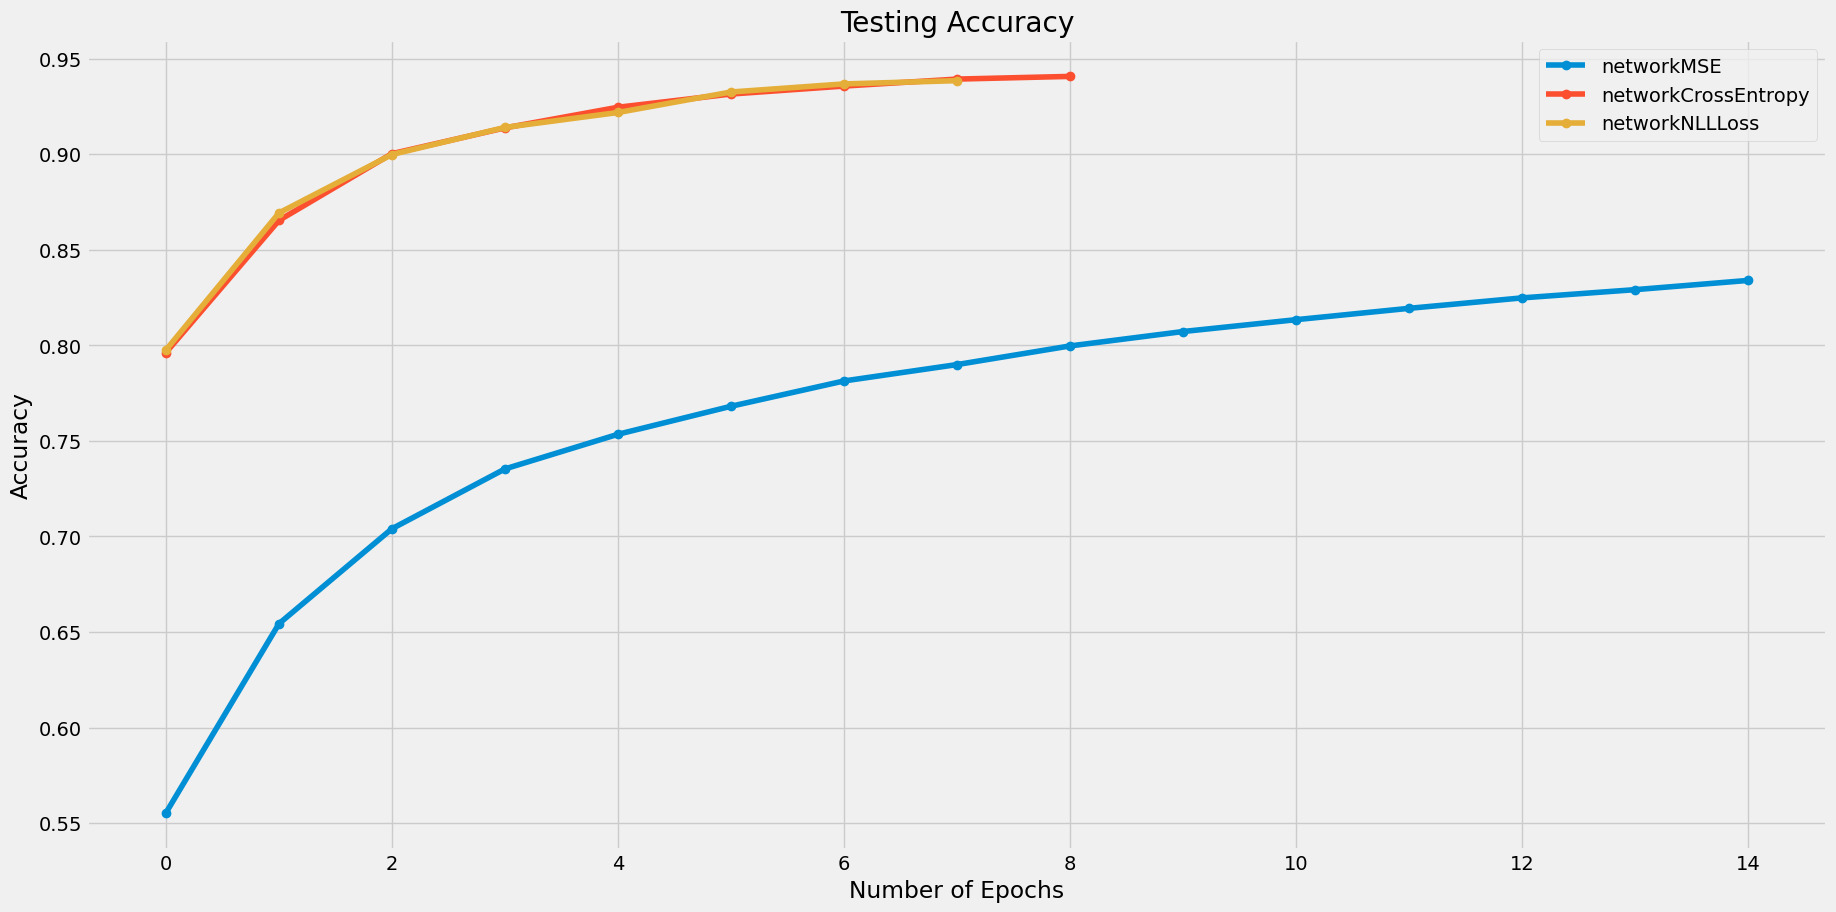
\includegraphics[scale=0.3]{Loss Functions Accuracy}
    \caption{Loss functions with respect to overall model accuracy}
    \label{fig:nn_loss_function_accuracy}
\end{figure}

\begin{figure}[H]
    \centering
    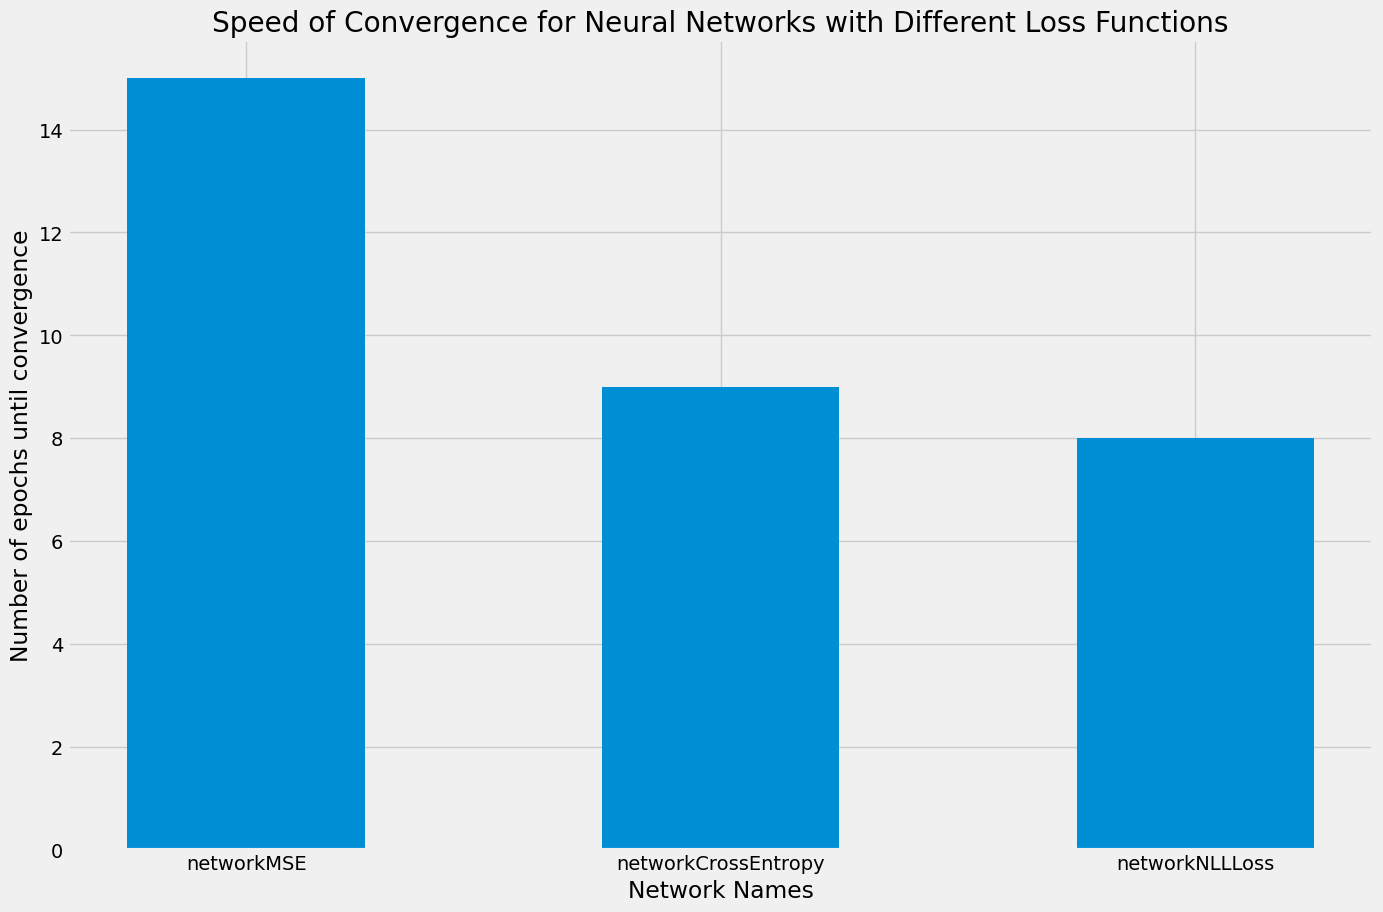
\includegraphics[scale=0.3]{Convergence Loss Functions}
    \caption{Loss functions with respect to model convergence}
    \label{fig:nn_loss_function_convergence}
\end{figure}

Given the performance shown in Figure \ref{fig:nn_loss_function_accuracy} and Figure \ref{fig:nn_loss_function_convergence}, it is pretty clear that the cross entropy and negative log likelihood loss functions can be used interchangeably as there's very a minor difference between the two. However, mean square error loss function is shown to be much worse in terms of accuracy as well as time taken to converge. This can be justified as MSE is mainly used in regression tasks to predict continuous values.
In the domain of classifying handwritten digits, the cross-entropy and NLL loss functions are typically more appropriate and yield better results due to their ability to optimize probability estimates of a class given a dataset.

\subsubsection{Activation Function Optimization}
Activation function optimization refers to the process of selecting or designing the most suitable activation function for each layer in a network. The choice of activation function plays a crucial role in the network's ability to learn and generalize from the data. Therefore, the effectiveness of different activation functions will be analysed.

\begin{figure}[H]
    \centering
    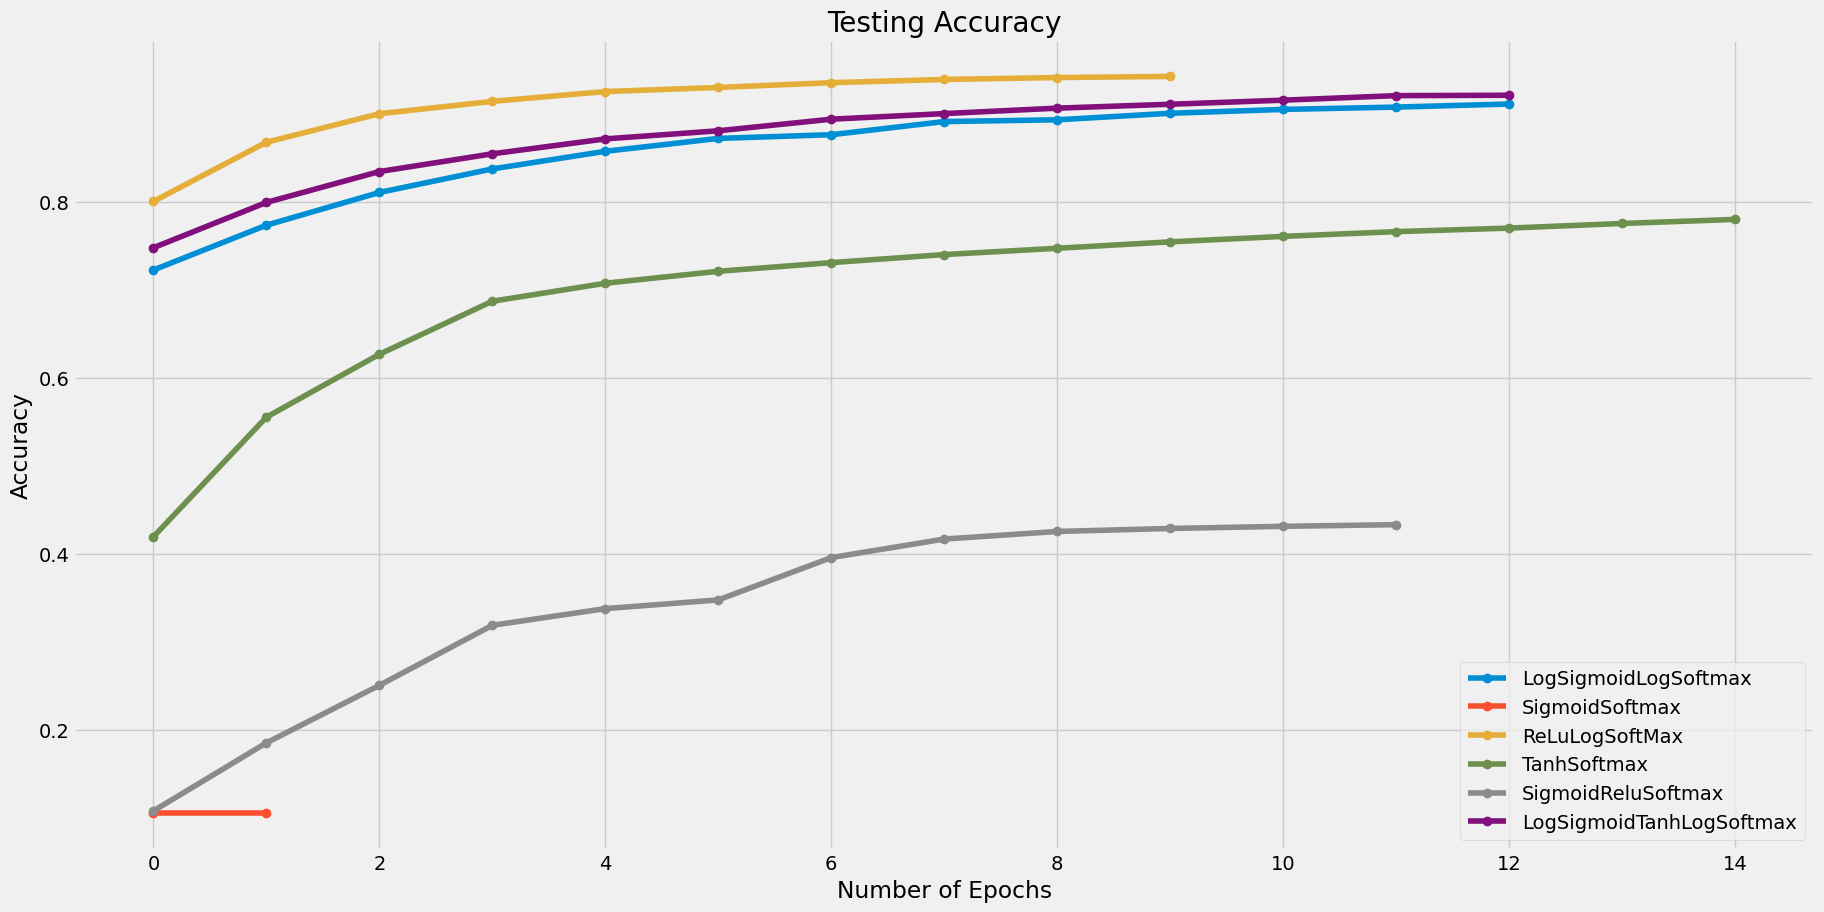
\includegraphics[scale=0.3]{Activation Functions Accuracy}
    \caption{Convergence with different activation functions}
    \label{fig:nn_activation_accuracy}
\end{figure}

\begin{figure}[H]
    \centering
    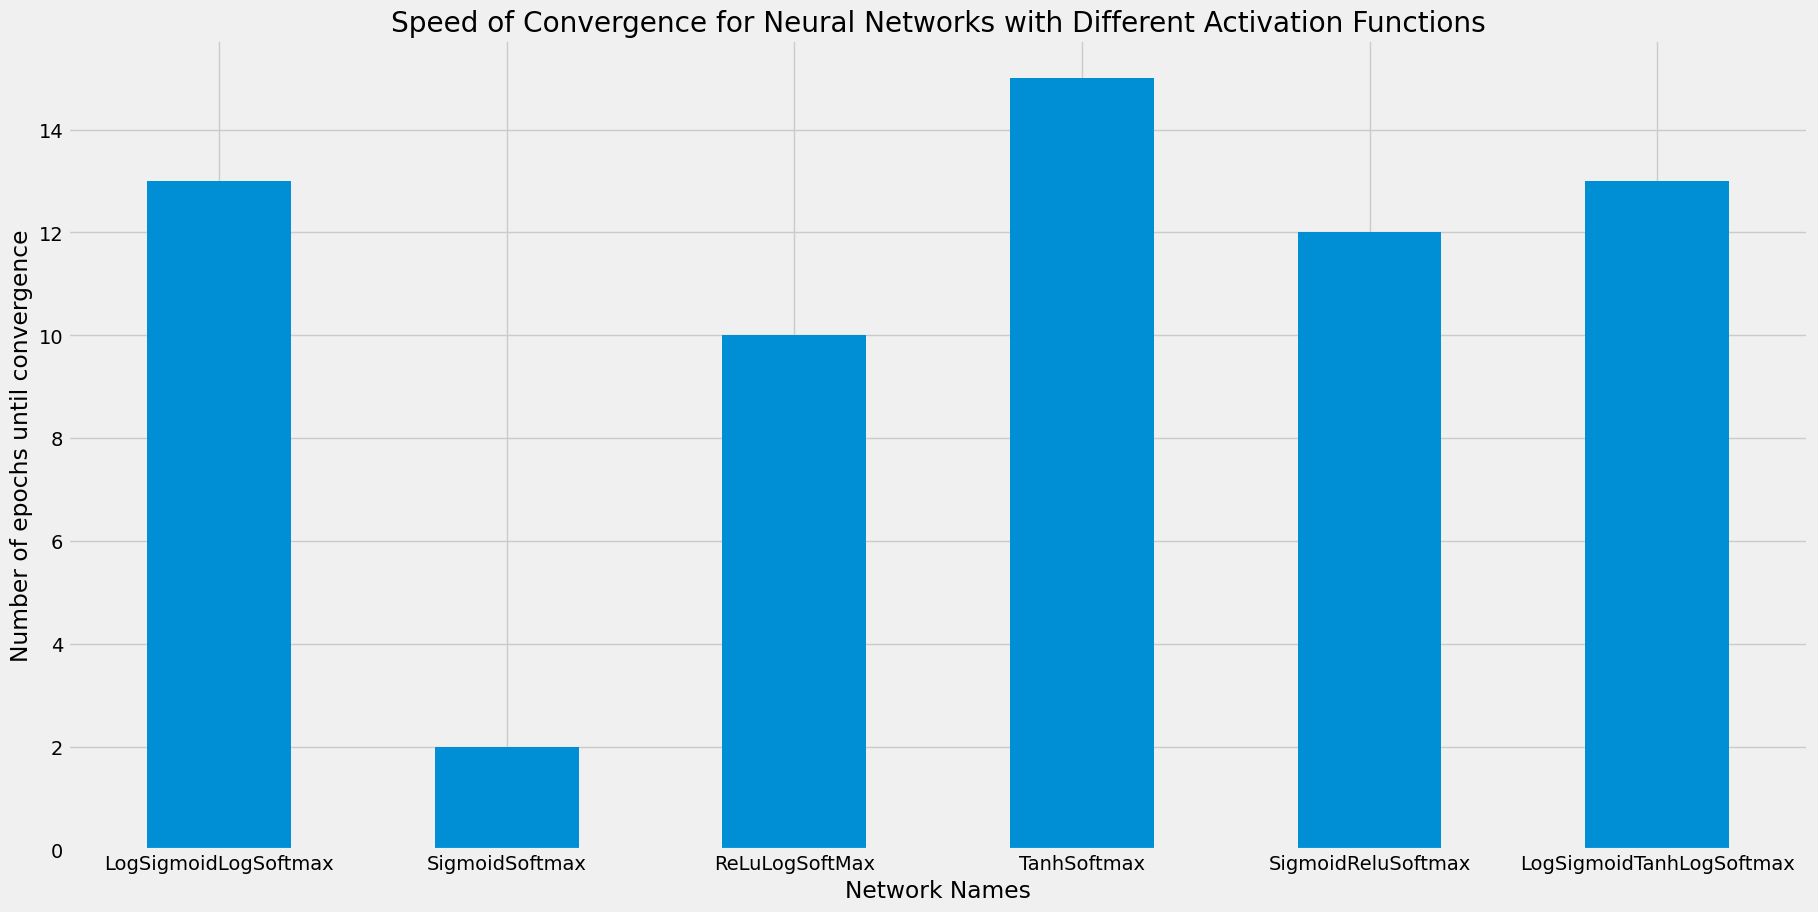
\includegraphics[scale=0.3]{Convergence Activation Functions}
    \caption{Convergence with different activation functions}
    \label{fig:nn_activation_convergence}
\end{figure}

As shown in Figure \ref{fig:nn_activation_accuracy} and Figure \ref{fig:nn_activation_convergence}, the softmax ReLu log function performed best overall. The softmax sigmoid activation function performed sub-optimally compared to the other activation functions. This could be due to:

\begin{itemize}
    \item \textbf{Vanishing/Exploding Gradients:} The vanishing gradient problem can affect the softmax and sigmoid activation functions, particularly in deep networks. When gradients become very small during back-propagation, the weights of the network may not be updated efficiently, resulting in sluggish learning and poor convergence to the optimal solution.

    \item \textbf{Limited Discriminative Power:} Softmax and sigmoid functions can be limited in their ability to capture complex non-linear decision limits. They may struggle to effectively model complex relationships in the data, resulting in low discriminative power and accuracy.

    \item \textbf{Hyper-parameter issues:} Inadequate tuning of hyper-characteristics like learning rate, regularization strength, or network design parameters can also have an effect on accuracy. In some circumstances, rapid convergence may be caused by hyper-parameters that are set excessively high, allowing the network to oversimplify the problem and result in sub-optimal accuracy.
\end{itemize}

\subsubsection{Optimizer performance}
Optimizers play a critical role in neural network training and are critical for achieving good performance. We will now analyze the performance of different optimizers.

\begin{figure}[H]
    \centering
    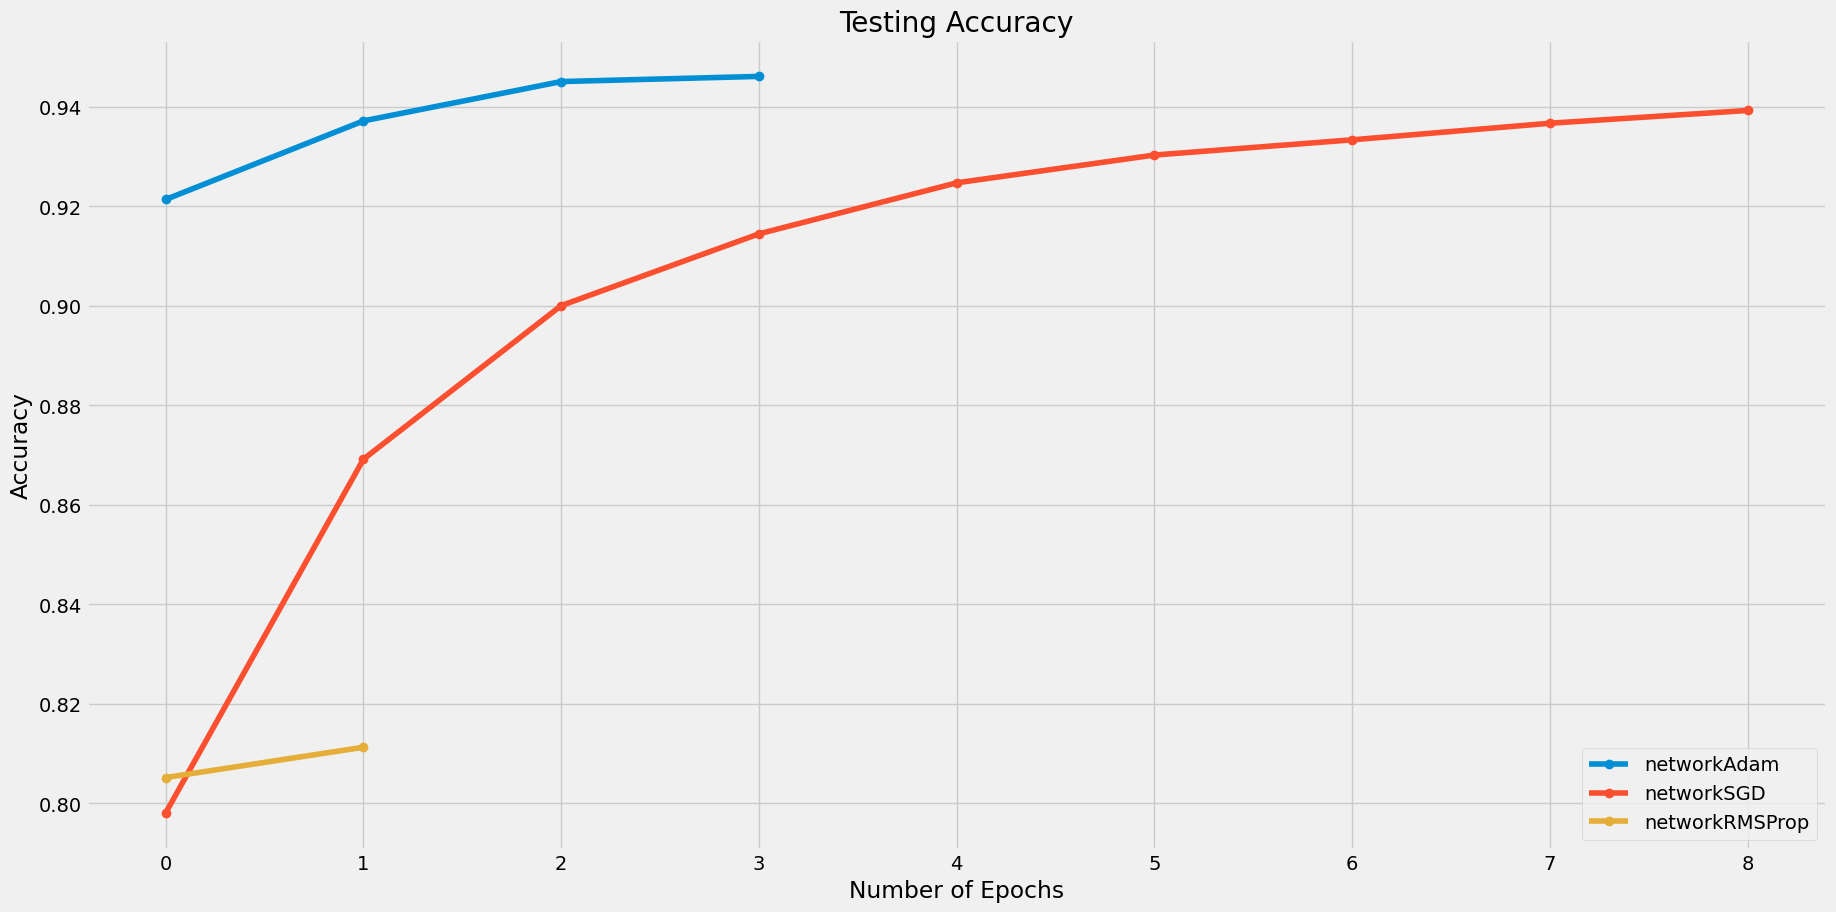
\includegraphics[scale=0.3]{Optimizers Accuracy}
    \caption{Accuracy with different optimizers}
    \label{fig:nn_optimizer_accuracy}
\end{figure}

\begin{figure}[H]
    \centering
    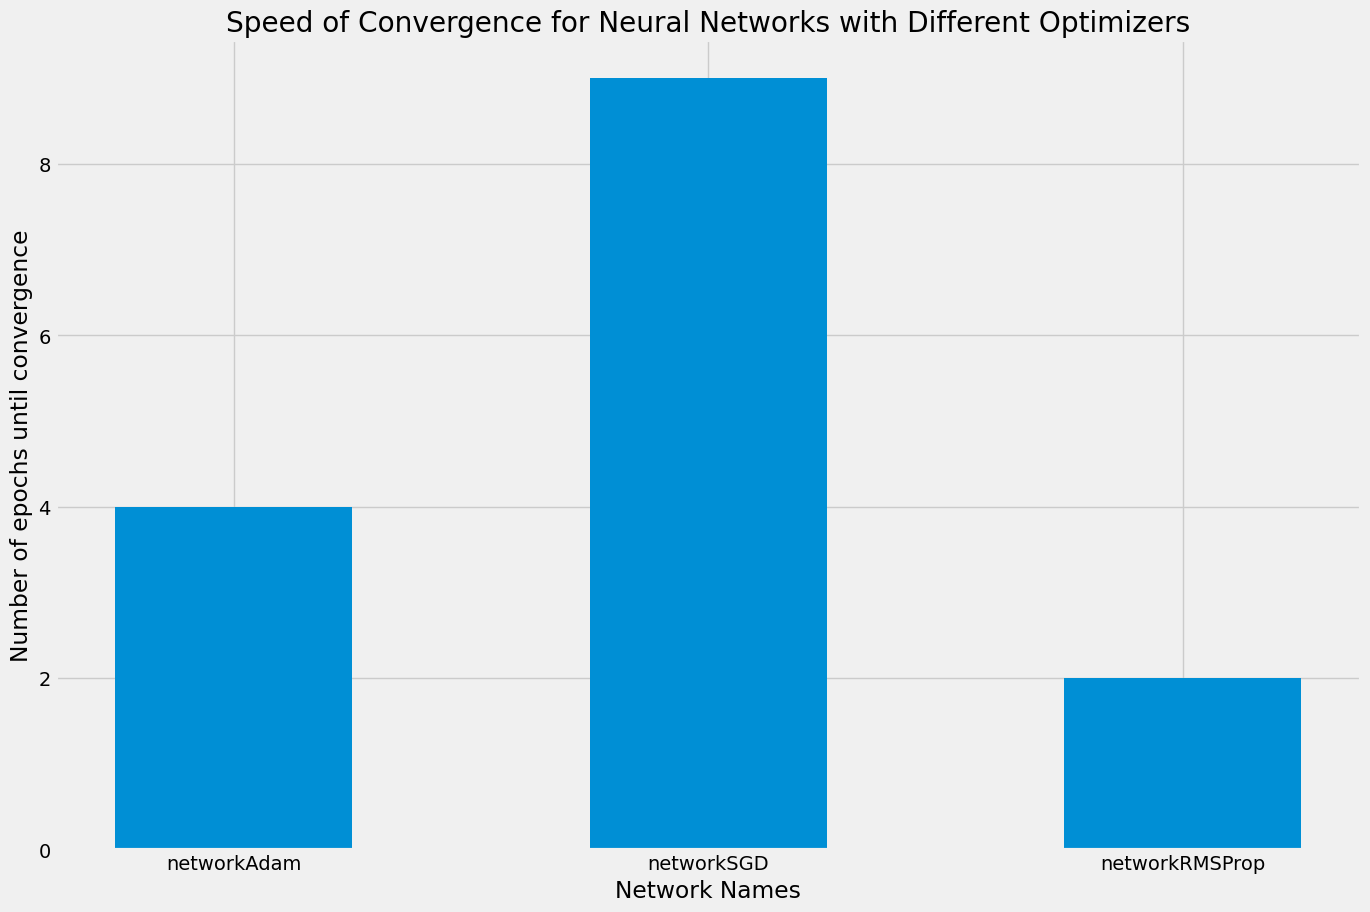
\includegraphics[scale=0.3]{Convergence Optimizers}
    \caption{Convergence with different optimizers}
    \label{fig:nn_optimizer_convergence}
\end{figure}

The adam optimizer is shown to produce the best combination of accuracy and convergence speed. This could be due to a characteristics of the data-set, different optimization strategies may have variable degrees of success. Some problems may benefit from Adam's adaptive learning rate, while others may require entirely different optimization strategies. It seems in the case of handwritten digits, the adaptive learning rate is more crucial for a balance between convergence speed and accuracy.  

\subsection{Convolutional Neural Network}
CNNs capture spatial hierarchies in data naturally. The network's early layers capture low-level characteristics, whereas later layers catch more complicated and abstract features. This hierarchical structure corresponds to the hierarchical structure of visual information, allowing CNNs to grasp and display data in a manner similar to human perception.

We will now explore the effectiveness of a convolutional neural network in identifying handwritten digits. Convolutional neural networks are particularly effective for tasks involving analysis and processing of structured grid-like data, such as images and videos. We won't repeat the same experiments as done for regular Neural Networks as they yield similar results due to the nature of the data. 

\subsubsection{Model structure}
The structure of the network is as follows:
\begin{itemize}
    \item \textbf{Convolution:} The input will be a $28 \times 28$ image padded $2$ pixels thick and has a $5 \times 5$ kernel convoluted to it. This convolution results in $6$ channels. $1 \times 28 \times 25$ padded $\rightarrow$ $(1 \times 32 \times 32 * 5 \times 5)$ $\rightarrow$ $6 \times 28 \times 28$

    \item \textbf{Pooling:} Those channels will go through a tanh activation function then will be down-sampled with an average pooling layer with kernel size $2 \times 2$. Down sampling average pooling $\rightarrow$ $6 \times 14 \times 14$

    \item \textbf{Convolution:} Those channels will not be padded and will have $5 \times 5$ kernels convoluted to them. This convolution will result in $16$ channels. $6 \times 14 \times 14 * 5 \times 5 \rightarrow 16 \times 10 \times 10$
    

    \item \textbf{Pooling:} Those channels will go through another tanh activation function, and then will be down sampled with an average pooling later with kernel size $2 \times 2$.
    Down sampling average pooling $\rightarrow 16 \times 5 \times 5$

    \item \textbf{Convolution:} Those channels will not be padded, and will have $5 \times 5$ kernel convoluted to them. This convolution will result in $120$ channels. $16 \times 5 \times 5 * 5 \times 5 \rightarrow 120 \times 1 \times 1$
    

    \item \textbf{Remaining layers:} Those channels will then go through a tanh activation function and flattened to $120$ nodes. They will once again go through a tanh activation function to $84$ nodes. Those $84$ nodes will be connected to the $10$ output nodes with no activation function. The loss function will be based on the cross entropy loss function. The CNN uses the adam optimizer.
\end{itemize}

The CNN has the following macro-performance:
\begin{center}
\begin{tabular}{||c|c||}
    Accuracy & $0.9652$ \\
    Precision & $0.9652$ \\
    Sensitivity & $0.9654$ \\
    F1 Score & $0.9651$ \\
\end{tabular}
\end{center}

\begin{figure}[H]
    \centering
    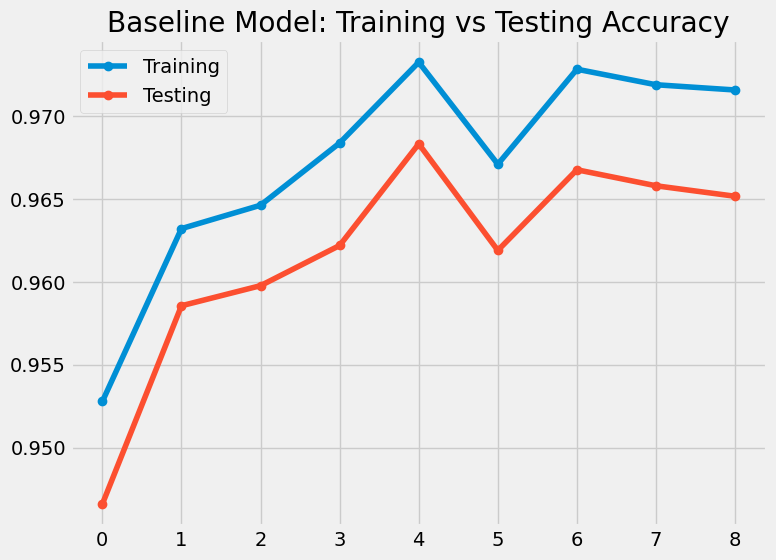
\includegraphics[scale=0.3]{Baseline CNN Acc}
    \caption{CNN Accuracy}
    \label{fig:cnn_accuracy}
\end{figure}

\begin{figure}[H]
    \centering
    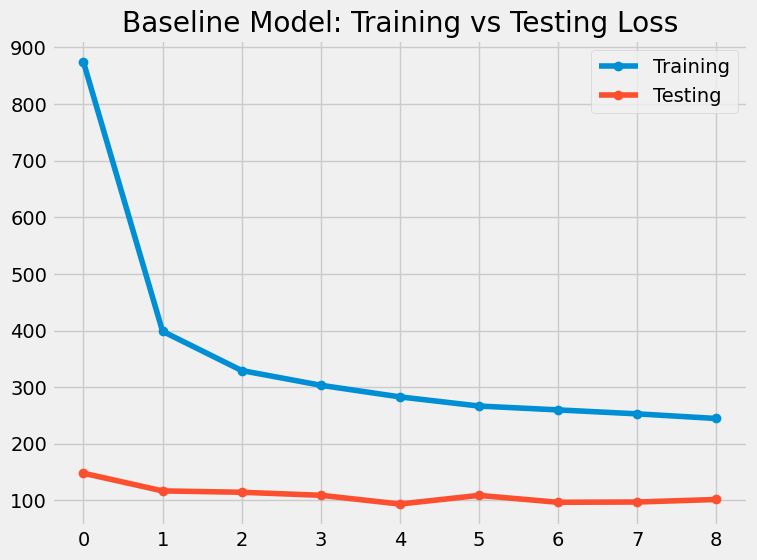
\includegraphics[scale=0.3]{Baseline CNN Loss}
    \caption{CNN Loss}
    \label{fig:cnn_loss}
\end{figure}

\begin{figure}[H]
    \centering
    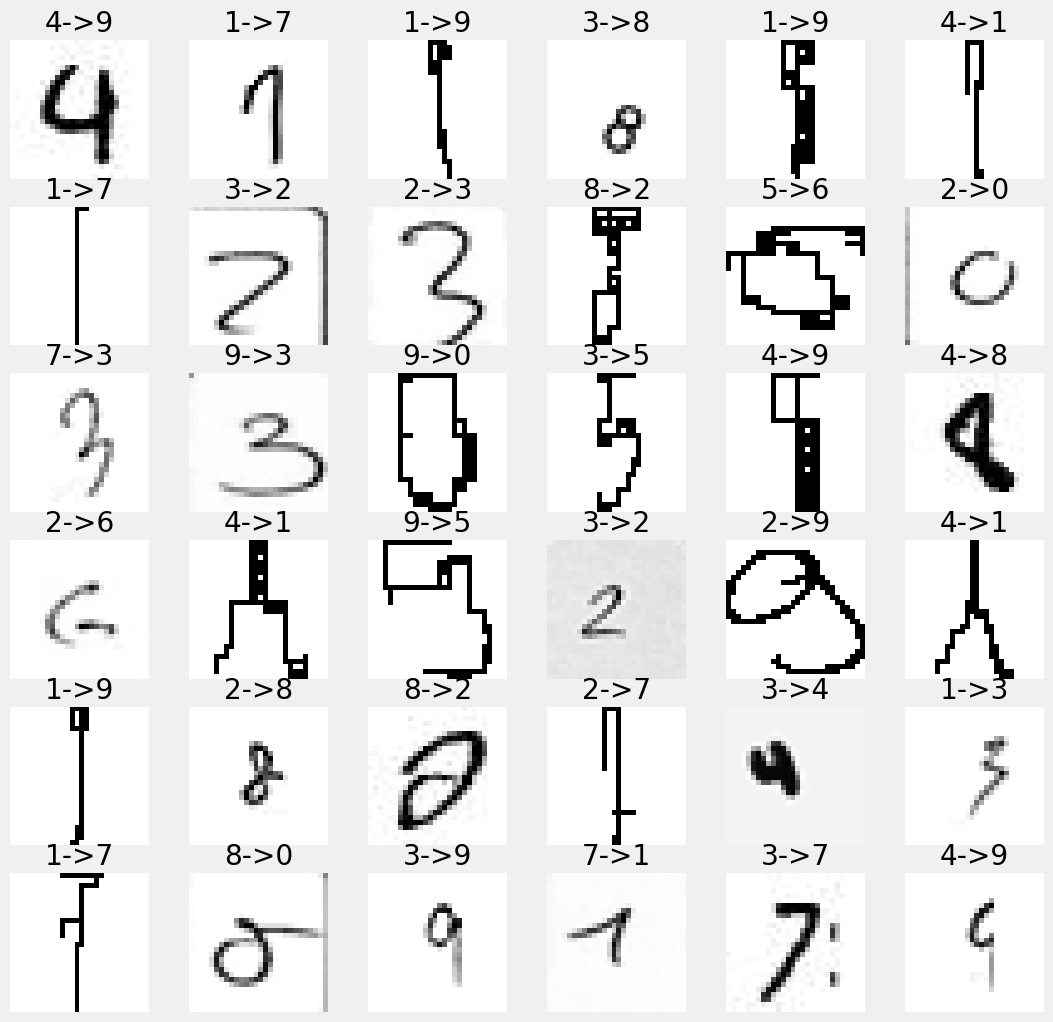
\includegraphics[scale=0.3]{Incorrect CNN}
    \caption{Incorrect classifications in the format prediction $\rightarrow$ actual}
    \label{fig:cnn_incorrect}
\end{figure}

Although the CNN shows minor improvement over the NN models, it is important to note that improving accuracy gets significantly difficult the closer a model is to $100\%$, based on the metrics shown about, it can be seen that a CNN provides a substantial improvement over NNs. 
We believe for the same reasons as training the NN before that refining the dataset further by removing illegible digits and adding additional legible datasets will allow the local spatial patterns to be better identified, allowing the CNN to perform better. The reason for this is the observed misclassifications by a CNN compared to the regular NN are that the noise in the illegible digits contribute to the spatial pattern being identified, as "8" and "9" seem to be the commonly misclassified datapoints.

\section{Conclusion}
This report evaluated Convolutional Neural Networks (CNNs) and conventional Neural Networks (NNs) for detecting handwritten digits. 

In conclusion, our project involved sourcing multiple handwritten datasets to create a comprehensive repository for training a neural network. The neural network demonstrated strong performance, achieving a high level of accuracy in classifying handwritten digits. Additionally, the utilization of a convolutional neural network (CNN) resulted in even better performance compared to other models.

However, we identified areas for potential improvement. Refining the datasets by excluding illegible or ambiguous samples could reduce noise and enhance the model's predictive capabilities. Additionally, introducing more legible datasets specifically for digits with similar stroke patterns, such as "0" and "9" or "2" and "3," could help the model differentiate between these challenging pairs.

For future work, it would be worthwhile to explore the impact of dataset quality on model accuracy. Improving the quality of the datasets may yield better model performance.

By addressing these aspects and focusing on dataset refinement and additions, we can continue to improve the accuracy and performance of the model for handwritten digit recognition.

\nocite{*}
\bibliography{references}\addcontentsline{toc}{chapter}{References}
\end{document}
